\documentclass[xcolor=pdflatex,dvipsnames,table]{beamer}
\usepackage{epsfig,graphicx}
\usepackage{palatino}
\usepackage{fancybox}
\usepackage{relsize}
\usepackage[procnames]{listings}
\usepackage{hyperref}
\usepackage{qtree} % needed?
\usepackage{booktabs}
\usepackage{dirtree}
\usepackage[normalem]{ulem}


% fatter TT font
\renewcommand*\ttdefault{txtt}
% another TT, suggested by Alex
% \usepackage{inconsolata}
% \usepackage[T1]{fontenc} % needed as well?


\newcommand{\scale}{0.7}

\newcommand{\todo}[1]{{\emph{TODO: #1}}}
\newcommand{\martin}[1]{{\color{blue} Martin: #1}}
\newcommand{\abcdef}[1]{{\color{red} Author2: #1}}

% uncomment following for final submission
%\renewcommand{\todo}[1]{}
%\renewcommand{\martin}[1]{}
%\renewcommand{\author2}[1]{}

\newcommand{\code}[1]{{\texttt{#1}}}

\hypersetup{
  linkcolor  = black,
%  citecolor  = blue,
  urlcolor   = blue,
  colorlinks = true,
}

\beamertemplatenavigationsymbolsempty
\setbeamertemplate{footline}[frame number]





\newif\ifbook
% shared in slides and book

\lstdefinelanguage{chisel}{
%  morekeywords={abstract,case,catch,class,def,%
%    do,else,extends,false,final,finally,%
%    for,if,implicit,import,match,mixin,%
%    new,null,object,override,package,%
%    private,protected,requires,return,sealed,%
%    super,this,throw,trait,true,try,%
%    type,val,var,while,with,yield},
%  otherkeywords={=>,<-,<\%,<:,>:,\#,@},
  sensitive=true,
  morecomment=[l]{//},
  morecomment=[n]{/*}{*/},
  morestring=[b]",
  morestring=[b]',
  morestring=[b]"""
}

\usepackage{color}
\definecolor{dkgreen}{rgb}{0,0.6,0}
\definecolor{gray}{rgb}{0.5,0.5,0.5}
\definecolor{mauve}{rgb}{0.58,0,0.82}

% Default settings for code listings
%\ifbook
\lstset{%frame=lines,
  language=chisel,
  aboveskip=3mm,
  belowskip=3mm,
  showstringspaces=false,
  columns=fixed, % basewidth=\mybasewidth,
  basicstyle={\small\ttfamily},
  numbers=none,
  numberstyle=\footnotesize,
  % identifierstyle=\color{red},
  breaklines=true,
  breakatwhitespace=true,
  procnamekeys={def, val, var, class, trait, object, extends},
  % procnamestyle=\ttfamily,
  tabsize=2,
  float
}
%\else
%\lstset{%frame=lines,
%  language=chisel,
%  aboveskip=3mm,
%  belowskip=3mm,
%  showstringspaces=false,
%  columns=fixed, % basewidth=\mybasewidth,
%  basicstyle={\small\ttfamily},
%  numbers=none,
%  numberstyle=\footnotesize\color{gray},
%  % identifierstyle=\color{red},
%  keywordstyle=\color{blue},
%  commentstyle=\color{dkgreen},
%  stringstyle=\color{mauve},
%  breaklines=true,
%  breakatwhitespace=true,
%  procnamekeys={def, val, var, class, trait, object, extends},
%  procnamestyle=\ttfamily\color{red},
%  tabsize=2,
%  float
%}
%\fi

\lstnewenvironment{chisel}[1][]
{\lstset{language=chisel,#1}}
{}

\newcommand{\shortlist}[1]{{\lstinputlisting[nolol]{#1}}}

\newcommand{\longlist}[3]{{\lstinputlisting[float, caption={#2}, label={#3}, frame=tb, captionpos=b]{#1}}}

\newcommand{\verylonglist}[3]{{\lstinputlisting[caption={#2}, label={#3}, frame=tb, captionpos=b]{#1}}}


\title{Outro}
\author{Martin Schoeberl}
\date{\today}
\institute{Technical University of Denmark\\
Embedded Systems Engineering}

\begin{document}

\begin{frame}
\titlepage
\end{frame}


\begin{frame}[fragile]{Overview}
\begin{itemize}
\item Evaluation
% \item Chisel from scratch
\item Who is Alan Turing?
\item Lipsi, a simple processor
\item Show VM today
\item Report hand-in at DTU Learn (24 May)
\item We have well known guest lectures today
\begin{itemize}
\item Tjark and Kasper will present today
\end{itemize}
\end{itemize}
\end{frame}


\begin{frame}[fragile]{The Online Exam}
\begin{itemize}
\item At \url{https://eksamen.dtu.dk/}
\item On Tuesday 18/5 10:00--12:00 (12:30)
\item It will be two parts:
\begin{itemize}
\item Multiple choice
\item Download and hand in a PDF document (e.g., generated from Word or photo taken)
\end{itemize}
\end{itemize}
\end{frame}


\begin{frame}[fragile]{Evaluation}
\begin{itemize}
%\item Thank you!
\item Looks like you enjoyed DE2 and Chisel :-)
\item Some found it to easy -- Maybe I should change that
\item Not so many answers, is there an evaluation fatigue?
\item Let us look into it
\end{itemize}
\end{frame}

%\begin{frame}[fragile]{Write in Chisel from Scratch}
%\begin{itemize}
%\item This was a request from the evaluation
%\item Should not be too hard
%\item We need just two files
%\begin{itemize}
%\item \code{build.sbt} for library dependencies
%\item One Scala file
%\end{itemize}
%\item Let's do it now!
%\end{itemize}
%\end{frame}

\begin{frame}[fragile]{FSMD}
\begin{itemize}
\item A finite-state machine and a datapath
\item Can compute
\item Your vending machine is an FSMD
\item Can we use this to build a general processor?
\end{itemize}
\end{frame}

\begin{frame}[fragile]{What is a \emph{General} Processor?}
\begin{itemize}
\item A computing machine that can compute all computable problems
\item What is computable?
\item Mr. \href{https://en.wikipedia.org/wiki/Alan_Turing}{Turing} thought about this before computers where built (1936)
\item The \href{https://en.wikipedia.org/wiki/Turing_machine}{Turing machine} can compute all computable problems
\item How useful is this?
\item What is NOT computable?
\item Assumption is infinite resources (memory)
\item But even with finite amount of memory it is a VERY useful classification
\end{itemize}
\end{frame}

\begin{frame}[fragile]{A Practical Turing-Complete Machine}
\begin{itemize}
\item Compute with some operations
\item Control 1: an FSM to steer the datapath
\item Control 2: instructions to steer the FSM
\item Storage: memory for the \emph{infinite/large} storage
\end{itemize}
\end{frame}

\begin{frame}[fragile]{Can We Build Such a Processor?}
\begin{itemize}
\item Our Chisel and digital design knowledge should be enough
\item Let's start with a simple one
\item An FSMD plus memory
\item As it is small, we  name it after a small island: Lipsi
\end{itemize}
\end{frame}

\begin{frame}[fragile]{Lipsi}
\begin{itemize}
\item The paper: \href{https://www.jopdesign.com/doc/lipsi.pdf}{Lipsi: Probably the Smallest Processor in the World}
\item Code: \href{https://github.com/schoeberl/lipsi}{The Chisel Code}
\item A simple Accumulator machine
\end{itemize}
\end{frame}


\begin{frame}[fragile]{Lipsi Datapath}
\begin{figure}
  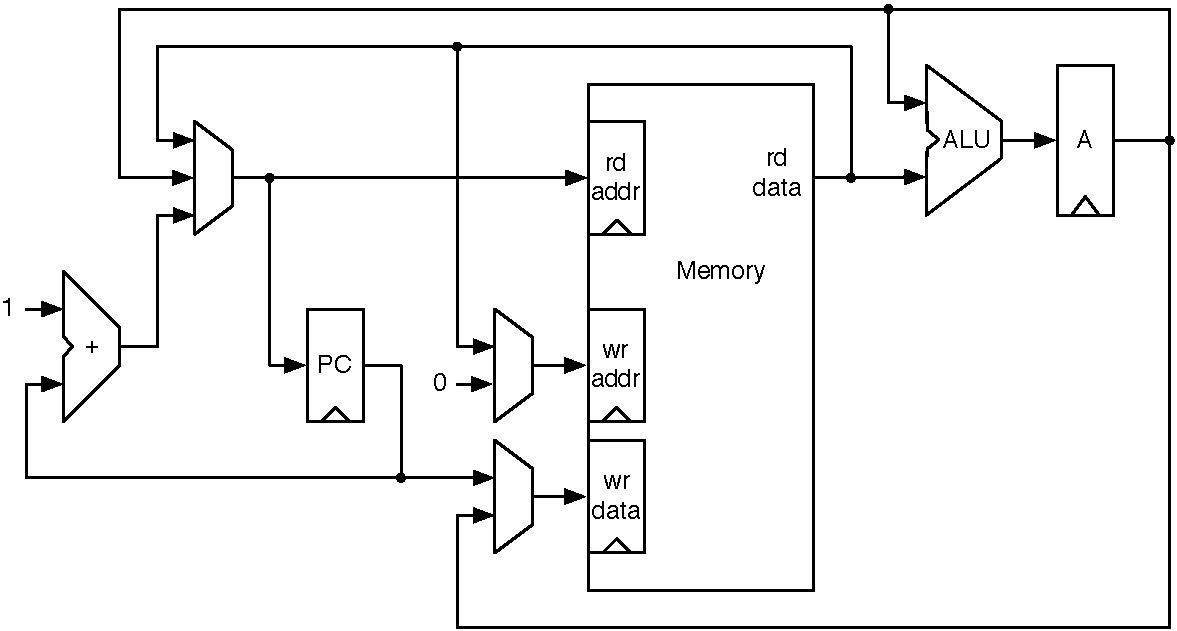
\includegraphics[scale=0.5]{../figures/lipsi}
\end{figure}
\end{frame}

\begin{frame}[fragile]{Datapath Elemenets}
\begin{itemize}
\item An arithmetic-logic unit (ALU)
\item An accumulator: register A
\item Memory for instructions and data
\item a program counter (PC)
\end{itemize}
\end{frame}

\begin{frame}[fragile]{Commanding the FSM}
\begin{itemize}
\item We need so-called instructions
\item They drive the FSM
\item To computer (e.g., +, -, or): ALU operations
\item To load from and store into memory
\item To (conditionally) branch (implement if/else, loops)
\end{itemize}
\end{frame}

\begin{frame}[fragile]{Lipsi Instruction Set}
{\footnotesize
\begin{table}
\begin{tabular}{lllll}
\toprule
Encoding & & Instruction & Meaning & Operation \\
\midrule
\code{0fff rrrr} & & $f$ rx & ALU register & A = A $f$ m[r]\\
\code{1000 rrrr} & & st rx & store A into register & m[r] = A\\
\code{1001 rrrr} & & brl rx & branch and link & m[r] = PC, PC = A\\
\code{1010 rrrr} & & ldind (rx) & load indirect & A = m[m[r]]\\
\code{1011 rrrr} & & stind (rx) & store indirect &m[m[r]] = A\\
\code{1100 -fff} & \code{nnnn nnnn} & $fi$ n & ALU immediate & A = A $f$ n\\
\code{1101 --00} & \code{aaaa aaaa} & br & branch & PC = a\\
\code{1101 --10} & \code{aaaa aaaa} & brz & branch if A is zero & PC = a\\
\code{1101 --11} & \code{aaaa aaaa} & brnz & branch if A is not zero & PC = a\\
\code{1110 --ff} & & sh &ALU shift & A = shift(A)\\
\code{1111 aaaa} & & io & input and output & IO = A, A = IO \\
\code{1111 1111} & & exit & exit for the tester & PC = PC\\
\bottomrule
\end{tabular}
\end{table}
}
\end{frame}

\begin{frame}[fragile]{ALU Operations}
\begin{table}
\begin{tabular}{lll}
\toprule
Encoding & Name & Operation \\
\midrule
\code{000} & add & $A = A + op$\\
\code{001} & sub & $A = A - op$\\
\code{010} & adc & $A = A + op + c$\\
\code{011} & sbb & $A = A - op - c$\\
\code{100} & and & $A = A \wedge op$\\
\code{101} & or & $A = A \vee op$\\
\code{110} & xor & $A = A \oplus op$\\
\code{111} & ld & $A = op$\\
\bottomrule
\end{tabular}
\end{table}
\end{frame}

\begin{frame}[fragile]{The ALU}
\begin{chisel}
  val add :: sub :: adc :: sbb :: and :: or :: xor :: ld :: Nil = Enum(8)
  switch(funcReg) {
    is(add) { res := accuReg + op }
    is(sub) { res := accuReg - op }
    is(adc) { res := accuReg + op } // TODO: adc
    is(sbb) { res := accuReg - op } // TODO: sbb
    is(and) { res := accuReg & op }
    is(or) { res := accuReg | op }
    is(xor) { res := accuReg ^ op }
    is(ld) { res := op }
  }
\end{chisel}
\end{frame}


\begin{frame}[fragile]{Some Defaults}
\begin{chisel}
  wrEna := false.B
  wrAddr := rdData
  rdAddr := Cat(0.U(1.W), nextPC)
  updPC := true.B
  nextPC := pcReg + 1.U
  enaAccuReg := false.B
  enaPcReg := false.B
  enaIoReg := false.B
\end{chisel}
\end{frame}


\begin{frame}[fragile]{Conditions for Branches}
\begin{chisel}
  val accuZero = accuReg === 0.U

  val doBranch = (rdData(1, 0) === 0.U) ||
    ((rdData(1, 0) === 2.U) && accuZero) ||
    ((rdData(1, 0) === 3.U) && !accuZero)
\end{chisel}
\end{frame}

\begin{frame}[fragile]{The FSM States and Register}
\begin{chisel}
  val fetch :: execute :: stind :: ldind1 :: ldind2 :: exit :: Nil = Enum(6)
  val stateReg = RegInit(fetch)
\end{chisel}
\end{frame}


\begin{frame}[fragile]{A Large State Machine}
\begin{chisel}
  switch(stateReg) {
    is(fetch) {
      stateReg := execute
      funcReg := rdData(6, 4)
      // ALU register
      when(rdData(7) === 0.U) {
        updPC := false.B
        funcReg := rdData(6, 4)
        enaAccuReg := true.B
        rdAddr := Cat(0x10.U, rdData(3, 0))
      }
      // st rx, is just a single cycle
      when(rdData(7, 4) === 0x8.U) {
        wrAddr := Cat(0.U, rdData(3, 0))
        wrEna := true.B
        stateReg := fetch
      }
    ...
\end{chisel}
\end{frame}



\begin{frame}[fragile]{Memory}
\begin{itemize}
\item Code memory for instructions
\item Data memory for data
\item Merge those two
\item Instruction memory filled by a program
\item That program is an assembler written in Scala
\end{itemize}
\end{frame}

\begin{frame}[fragile]{Code and Data Memory}
\begin{chisel}
  val program = VecInit(util.Assembler.getProgram(prog).map(_.U))
  val instr = program(rdAddrReg(7, 0))

  val mem = Mem(256, UInt(8.W))
  val data = mem(rdAddrReg(7, 0))
  when(io.wrEna) {
    mem(io.wrAddr) := io.wrData
  }
  
  // Output MUX
  io.rdData := Mux(rdAddrReg(8), data, instr)
\end{chisel}
\end{frame}


\begin{frame}[fragile]{An Assembly Program Example}
\begin{itemize}
\item Digital hardware and processors only understand 0 and 1
\item But, we do not want to program in 0s and 1s
\item We write in \href{https://en.wikipedia.org/wiki/Assembly_language}{assembly language}
\end{itemize}
\begin{chisel}
ldi 0x12
st r1
ldi 0x34
st r2
ldi 0
add r1
add r2
# now it is 0x46
\end{chisel}
\end{frame}

\begin{frame}[fragile]{Assembling Instructions}
\begin{chisel}
    for (line <- source.getLines()) {
      if (!pass2) println(line)
      val tokens = line.trim.split(" ")
      val Pattern = "(.*:)".r
      val instr = tokens(0) match {
        case "#" => // comment
        case Pattern(l) => if (!pass2) symbols += (l.substring(0, l.length - 1) -> pc)
        case "add" => 0x00 + regNumber(tokens(1))
        case "sub" => 0x10 + regNumber(tokens(1))
        case "adc" => 0x20 + regNumber(tokens(1))
        case "sbb" => 0x30 + regNumber(tokens(1))
        case "and" => 0x40 + regNumber(tokens(1))
        case "or" => 0x50 + regNumber(tokens(1))
\end{chisel}
This is done at hardware generation
\end{frame}



\begin{frame}[fragile]{Co-simulation for Testing}
\begin{itemize}
\item Write an implementation of Lipsi in Scala
\item This is an instruction set simulator, not hardware
\item This is your golden model
\item Run programs on the simulator and in the Chisel hardware
\item Compare the results (the value in the accumulator)
\end{itemize}
\end{frame}

\begin{frame}[fragile]{A Processor Summary}
\begin{itemize}
\item This is a tiny processor as an example
\item Chisel is productive: this was all done in 14 hours!
\item Kind of useful for small systems
\item You could implement your vending machine on it
\item Is this the way a general processor is built?
\item Not today, we use something called pipelining
\item You can learn this in:
\begin{itemize}
\item 02155: Computer Architecture and Engineering
\end{itemize}
\end{itemize}
\end{frame}

\begin{frame}[fragile]{02155: Computer Architecture and Engineering}
\begin{itemize}
\item Given by Alberto and me
\item \href{http://www2.imm.dtu.dk/courses/02155/}{Course description}
\item Learn how a real-world processor work
\item Learn the language of the machine (instructions)
\item Virtual memory and caches
\item We use RISC-V, the free instruction set
\item Project: write a simulator for the RISC-V
\begin{itemize}
\item In any language, may be in Chisel
\item May even be a full implementation in an FPGA
\end{itemize}
\item You can also do a complete RISC-V in an FPGA in a Fagproject
\end{itemize}
\end{frame}

\begin{frame}[fragile]{Future with Digital Design Education}
\begin{itemize}
\item There are several companies in DK doing chip design
\item FPGAs are available in the cloud
\begin{itemize}
\item To speedup computing
\item You can rent them from Amazon
\end{itemize}
\item Also FPGAs are used in embedded systems
\item Digital design is only part of a computer engineering education
\item But DTU does not have a clear path to a computer engineering education
\end{itemize}
\end{frame}



\begin{frame}[fragile]{Computer Engineering Education at DTU}
\begin{itemize}
\item On the interaction between hardware and software
\item Very well payed jobs :-)
\item Not an easy choice at DTU
\begin{itemize}
\item No BSc available
\item Between EE and CS
\end{itemize}
\item Start with Bsc. in EE
\item Specialization in Indlejrede systemer og programmering
\begin{itemize}
\item 02155: Computer Architecture and Engineering
\item 02105: Algoritmer og datastrukturer
\end{itemize}
\item Continue as MSc. in Computer Science and Engineering
\item Specialization in
\begin{itemize}
\item Digital Systems
\item Embedded and Distributed Systems
\end{itemize}
\end{itemize}
\end{frame}

\begin{frame}[fragile]{Computer Engineering within the EE Bachelor}
\begin{itemize}
\item You get well educated in electronics
\item Add the software side to your education
\item Select some of the following courses
\begin{itemize}
\item 02155: Computer Architecture and Engineering
\item 02105: Algorithms and Data Structures 1
\item 02161: Software Engineering 1
\item 02159: Operating Systems
\item 02157: Functional Programming
\item 02141: Computer Science Modelling
\item 02110: Algorithms and Data Structures 2
\end{itemize}
\item See also \href{https://www.dtu.dk/da/english/Education/msc/Programmes/computer_science_and_engineering/Prerequisites}{Prerequisites for EE Bsc}
\end{itemize}
\end{frame}

\begin{frame}[fragile]{Digital Design within an EE Master}
\begin{itemize}
\item Not an obvious choice, as there is no specialization in digital systems
\item Select some of the following courses
\begin{itemize}
\item 02155: Computer Architecture and Engineering
\item 02203: Design of Digital Systems
\item 02211: Advanced Computer Architecture
\item 02205: VLSI Design
\item 02217: Design of Arithmetic Processors
\item 02204: Design of Asynchronous Circuits
\item 02209: Test of Digital Systems
\end{itemize}
\end{itemize}
\end{frame}

\begin{frame}[fragile]{Summary}
\begin{itemize}
\item You now know enough digital design to build any digital system
\item You may get better on it with practice
\item When you understand the principles you can easily learn Verilog or VHDL in days
\item Chisel may be the future for hardware design
\item You might apply for a job in silicon valley with your Chisel knowledge ;-)
\item Hope to see some of you in upcoming courses
\end{itemize}
\end{frame}



\end{document}

%\begin{frame}[fragile]{xxx}
%\begin{itemize}
%\item yyy
%\end{itemize}
%\end{frame}
